\documentclass[paper=letter,11pt]{scrartcl}

\KOMAoptions{headinclude=true, footinclude=false}
\KOMAoptions{DIV=14, BCOR=5mm}
\KOMAoptions{numbers=noendperiod}
\KOMAoptions{parskip=half}
\addtokomafont{disposition}{\rmfamily}
\addtokomafont{part}{\LARGE}
\addtokomafont{descriptionlabel}{\rmfamily}
%\setkomafont{pageheadfoot}{\normalsize\sffamily}
\setkomafont{pagehead}{\normalsize\rmfamily}
%\setkomafont{publishers}{\normalsize\rmfamily}
\setkomafont{caption}{\normalfont\small}
\setcapindent{0pt}
\deffootnote[1em]{1em}{1em}{\textsuperscript{\thefootnotemark}\ }


\usepackage{amsmath}
\usepackage[varg]{txfonts}
\usepackage[T1]{fontenc}
\usepackage{graphicx}
\usepackage{xcolor}
\usepackage[american]{babel}
% hyperref is needed in many places, so include it here
\usepackage{hyperref}

\usepackage{xspace}
\usepackage{multirow}
\usepackage{float}


\usepackage{braket}
\usepackage{bbm}
\usepackage{relsize}
\usepackage{tcolorbox}

\def\ketY{\ensuremath{\ket {\Psi}}}
\def\iGeV{\ensuremath{\textrm{GeV}^{-1}}}
%\def\mp{\ensuremath{m_{\textrm{proton}}}}
\def\rp{\ensuremath{r_{\textrm{proton}}}}
\def\me{\ensuremath{m_{\textrm{electron}}}}
\def\aG{\ensuremath{\alpha_G}}
\def\rAtom{\ensuremath{r_{\textrm{atom}}}}
\def\rNucl{\ensuremath{r_{\textrm{nucleus}}}}
\def\GN{\ensuremath{\textrm{G}_\textrm{N}}}
\def\ketX{\ensuremath{\ket{\vec{x}}}}
\def\ve{\ensuremath{\vec{\epsilon}}}


\def\ABCDMatrix{\ensuremath{\begin{pmatrix} A &  B  \\ C  & D \end{pmatrix}}}
\def\xyprime{\ensuremath{\begin{pmatrix} x' \\ y' \end{pmatrix}}}
\def\xyprimeT{\ensuremath{\begin{pmatrix} x' &  y' \end{pmatrix}}}
\def\xy{\ensuremath{\begin{pmatrix} x \\ y \end{pmatrix}}}
\def\xyT{\ensuremath{\begin{pmatrix} x & y \end{pmatrix}}}

\def\IMatrix{\ensuremath{\begin{pmatrix} 0 &  1  \\ -1  & 0 \end{pmatrix}}}
\def\IBoostMatrix{\ensuremath{\begin{pmatrix} 0 &  1  \\ 1  & 0 \end{pmatrix}}}
\def\JThree{\ensuremath{\begin{pmatrix}    0 & -i & 0  \\ i & 0  & 0 \\ 0 & 0 & 0 \end{pmatrix}}} 
\def\JTwo{\ensuremath{\begin{bmatrix}    0 & 0 & -i  \\ 0 & 0  & 0 \\ i & 0 & 0 \end{bmatrix}}}
\def\JOne{\ensuremath{\begin{bmatrix}    0 & 0 & 0  \\ 0 & 0  & -i \\ 0 & i & 0 \end{bmatrix}}}
\def\etamn{\ensuremath{\eta_{\mu\nu}}}
\def\Lmn{\ensuremath{\Lambda^\mu_\nu}}
\def\dmn{\ensuremath{\delta^\mu_\nu}}
\def\wmn{\ensuremath{\omega^\mu_\nu}}
\def\be{\begin{equation*}}
\def\ee{\end{equation*}}
\def\bea{\begin{eqnarray*}}
\def\eea{\end{eqnarray*}}
\def\bi{\begin{itemize}}
\def\ei{\end{itemize}}
\def\fmn{\ensuremath{F_{\mu\nu}}}
\def\fMN{\ensuremath{F^{\mu\nu}}}
\def\bc{\begin{center}}
\def\ec{\end{center}}
\def\nus{$\nu$s}

\def\adagger{\ensuremath{a_{p\sigma}^\dagger}}
\def\lineacross{\noindent\rule{\textwidth}{1pt}}

\newcommand{\multiline}[1] {
\begin{tabular} {|l}
#1
\end{tabular}
}

\newcommand{\multilineNoLine}[1] {
\begin{tabular} {l}
#1
\end{tabular}
}



\newcommand{\lineTwo}[2] {
\begin{tabular} {|l}
#1 \\
#2
\end{tabular}
}

\newcommand{\rmt}[1] {
\textrm{#1}
}


%
% Units
%
\def\m{\ensuremath{\rmt{m}}}
\def\GeV{\ensuremath{\rmt{GeV}}}
\def\pt{\ensuremath{p_\rmt{T}}}


\def\parity{\ensuremath{\mathcal{P}}}

\usepackage{cancel}
\usepackage{ mathrsfs }
\def\bigL{\ensuremath{\mathscr{L}}}

\usepackage{ dsfont }



\usepackage{fancyhdr}
\fancyhf{}


\lhead{\Large 33-444} % \hfill Introduction to Particle Physics \hfill Spring 2020}
\chead{\Large Introduction to Particle Physics} % \hfill Spring 2020}
\rhead{\Large Spring 2020} % \hfill Introduction to Particle Physics \hfill Spring 2020}

\begin{document}
\thispagestyle{fancy}

\begin{center}
{\huge \textbf{Lecture 22}}
\end{center}

{\fontsize{14}{16}\selectfont


Play same game as last lecture to calculate ratios of cross sections

\begin{minipage}{0.6\textwidth}
\be
\sigma = \frac{1}{2E_1} \frac{1}{2E_2} |M|^2 d\Pi_{LIPS}
\ee
\end{minipage} \hfill
\begin{minipage}{0.3\textwidth}
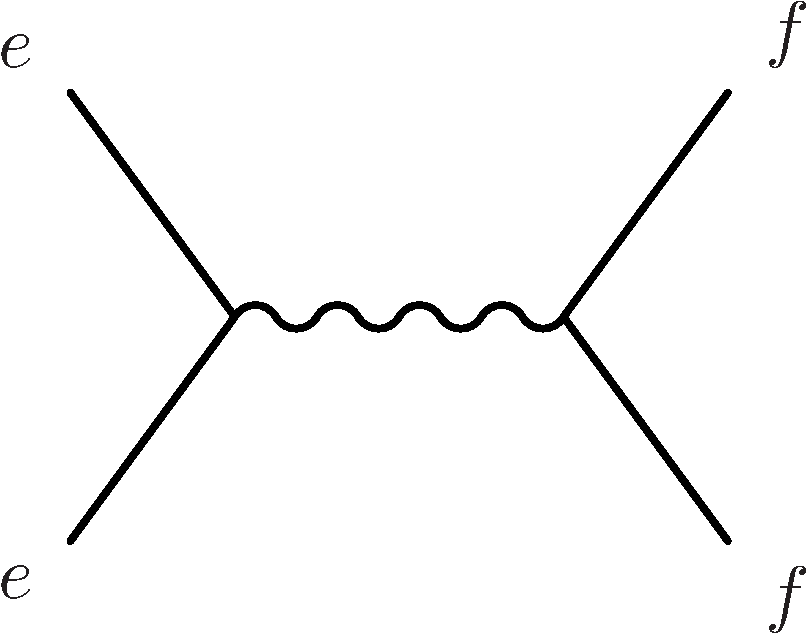
\includegraphics[width=0.8\textwidth]{./eeToff.pdf}
\end{minipage} 



\be
\frac{\sigma(ee\rightarrow \rmt{``jets''})}{\sigma(ee\rightarrow \mu\mu)} = \frac{\sum_{\rmt{``quarks''}} \sum_{\rmt{``colors''}} |M(ee\rightarrow qq)|^2  }{ \underbrace{|M(ee\rightarrow \mu\mu)|^2}_{|M_0|^2}}
\ee

\be
|M(ee\rightarrow qq)|^2 = Q_q^2 |M_0|^2
\ee

Define,
\be
R \equiv \frac{\sigma(ee\rightarrow \rmt{``jets''})}{\sigma(ee\rightarrow \mu\mu)} = \sum_{\rmt{quarks}} Q_q^2
\ee

R is sensitive to the number of quarks.


$R(E_{CM})$ at 4 GeV only u,d,s can contribute.

\be
R(E_{CM} < 4\ \rmt{GeV}) = \sum_{q \in\ u,d,s} Q_q^2 = \frac{4}{9} + \frac{1}{9} + \frac{1}{9} = \frac{2}{3}
\ee


\be
R(E_{CM} > 4\ \rmt{GeV}) = \sum_{q \in\ u,d,s,c} Q_q^2 = \frac{4}{9} + \frac{1}{9} + \frac{1}{9} + \frac{4}{9} = \frac{10}{9}
\ee

\clearpage

Problem, when you measure R you actually see

\bc
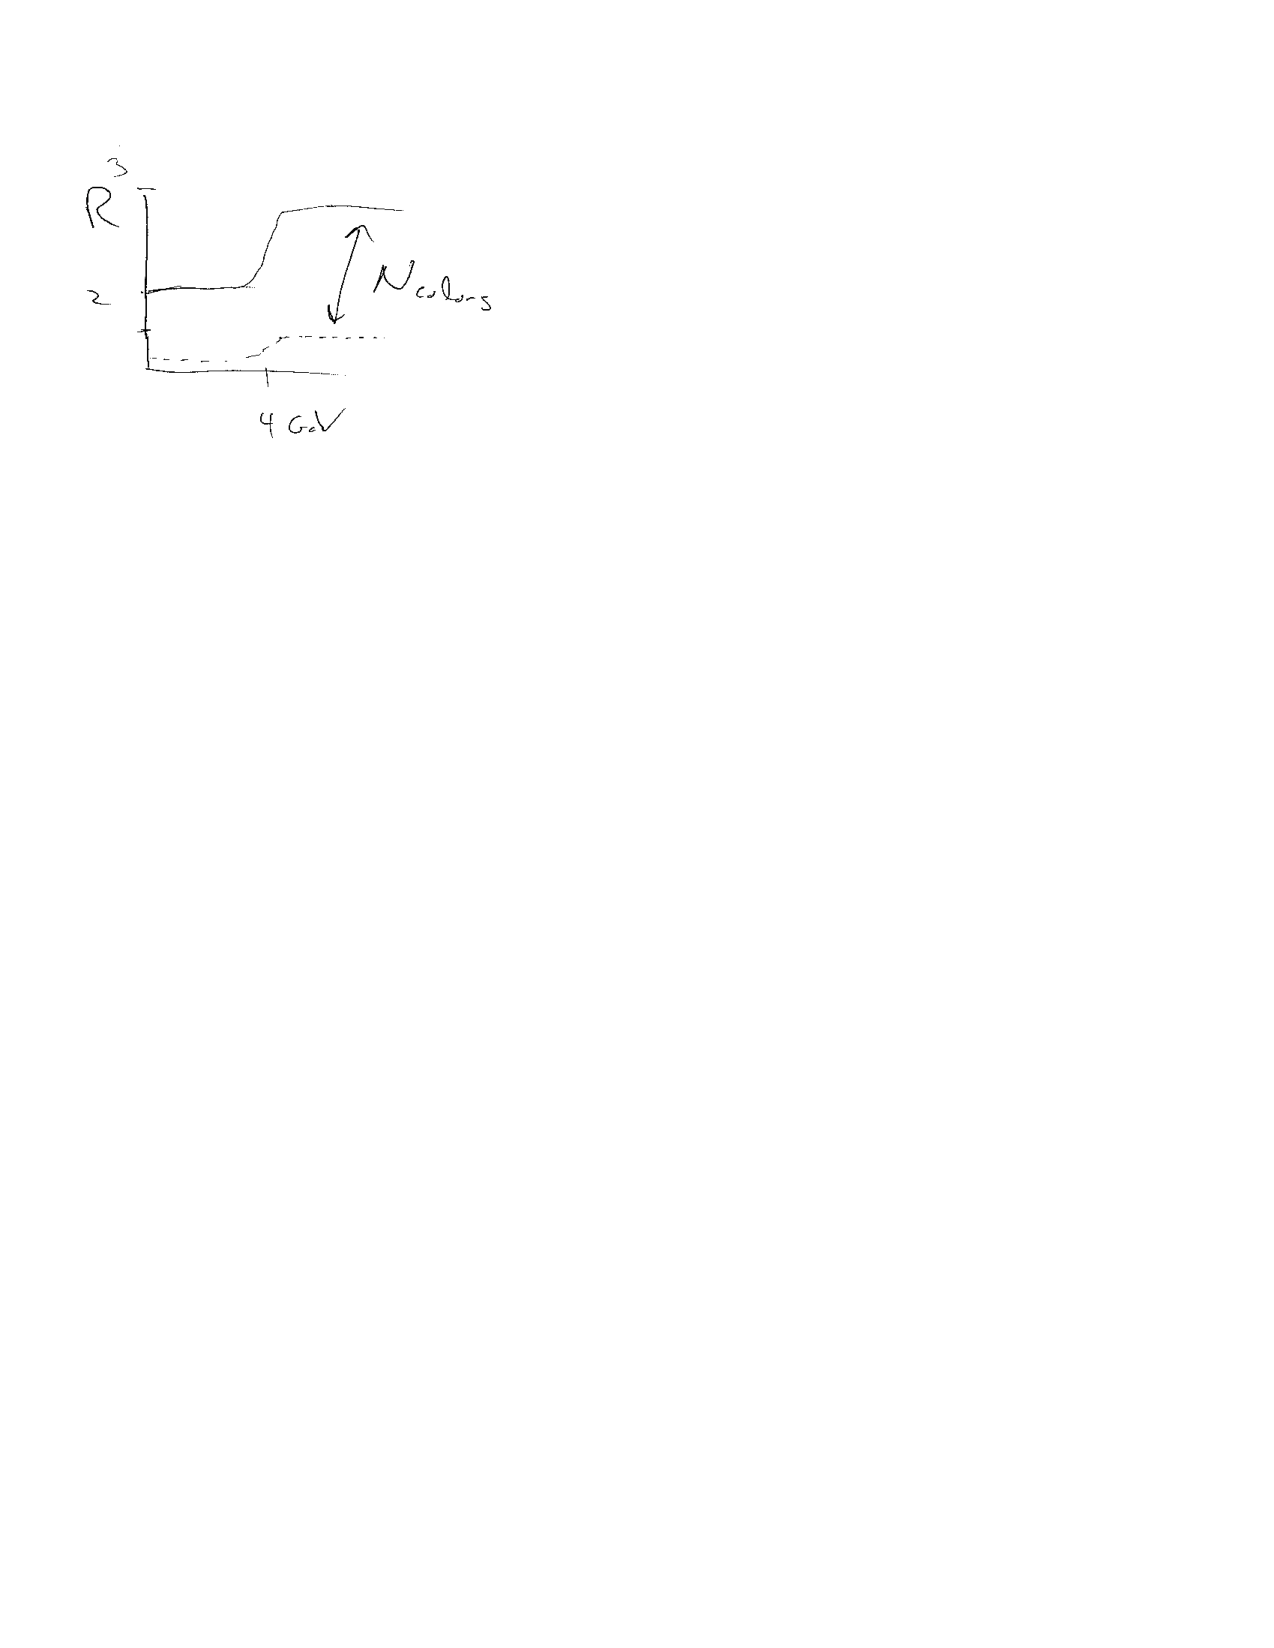
\includegraphics[width=0.8\textwidth]{./ObservedR.pdf}
\ec

Measuring R determines N$_{\rmt{quarks}}$ and N$_{\rmt{colors}}$.

Scan $E_{CM}$ measure R, changes at values of $m_q$.


\underline{Discovery of the gluon}

Cant produce glues from e's, but you can radiate them from q's produced in $ee\rightarrow qq$ collisions.
``Mercedes'' events smoking gun for gluons.

\begin{minipage}{0.5\textwidth}
\bc
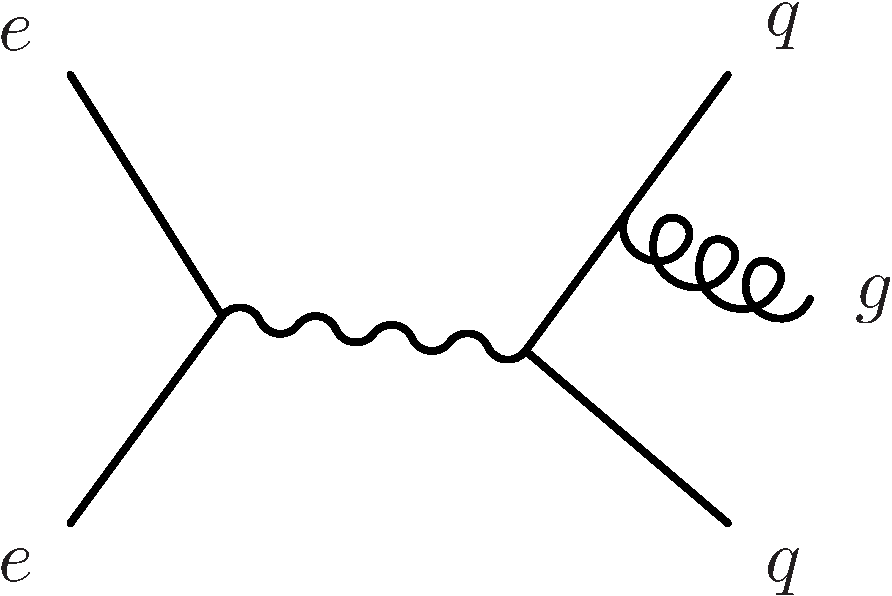
\includegraphics[width=0.6\textwidth]{./eeToqqg.pdf}
\ec
\be
\frac{\sigma(ee\rightarrow \rmt{3-jets})}{\sigma(ee\rightarrow \rmt{2-jets})} \sim \alpha_s N_{\rmt{gluons}}
\ee
\end{minipage} \hfill
\begin{minipage}{0.5\textwidth}
\bc
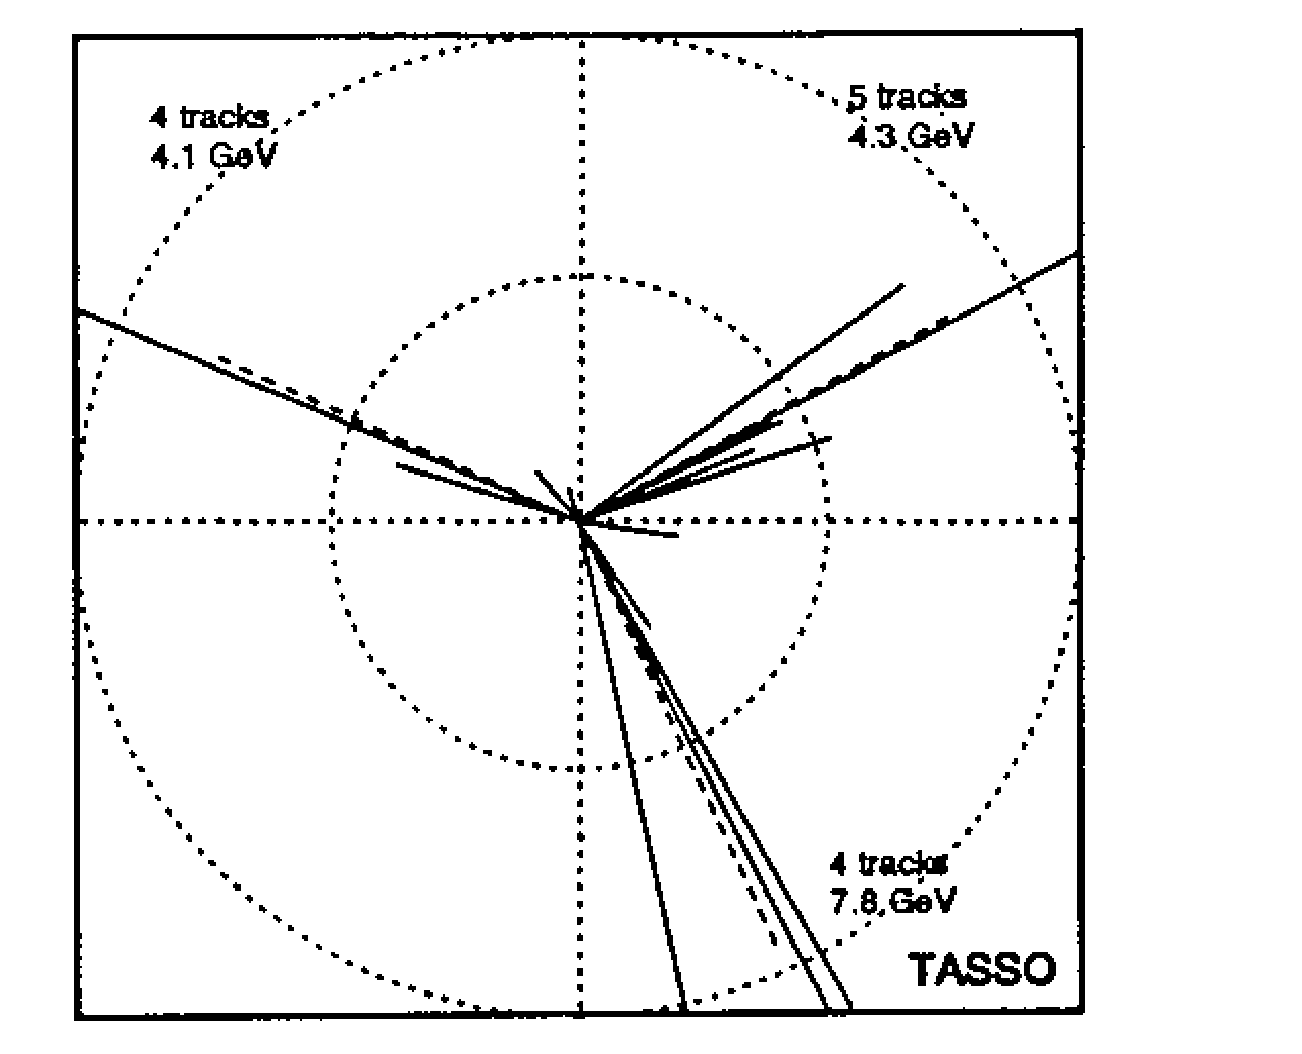
\includegraphics[width=0.8\textwidth]{./Tasso-3jet.png}
\ec
\end{minipage} \hfill

\clearpage 

Now collider physics in more detail.

Collide protons /  Measure how often a certain type of interaction occurs.

(Weve already talked about this...)

\be
r_p \sim GeV^{-1} \sim 10^{-15}m 
\ee


\be
r_p^2 \sim 10^{-26} cm^2 = 0.01\ \underbrace{\rmt{``barns''}}_{\rmt{Long story}}
\ee

barn is about the size of a Uranium atom.

At the LHC, interesting processes are
\bi
\item[-] nanobarns ($\sim 10^{-9}$ b)
\item[-] picobarns ($\sim 10^{-12}$ b)
\item[-] femptobarns ($\sim 10^{-15}$ b)
\ei 

One of the few units in particles physics not in natural units.

\lineacross

Now, colliding protons is \underline{\underline{hard}}.

- In order to get two protons to interact need to get them with an $fm \sim 10^{-15}m$ of each other.
- To get around this, we collide bunches of protons \\
Bunch is $\sim 10^{11}$ protons 

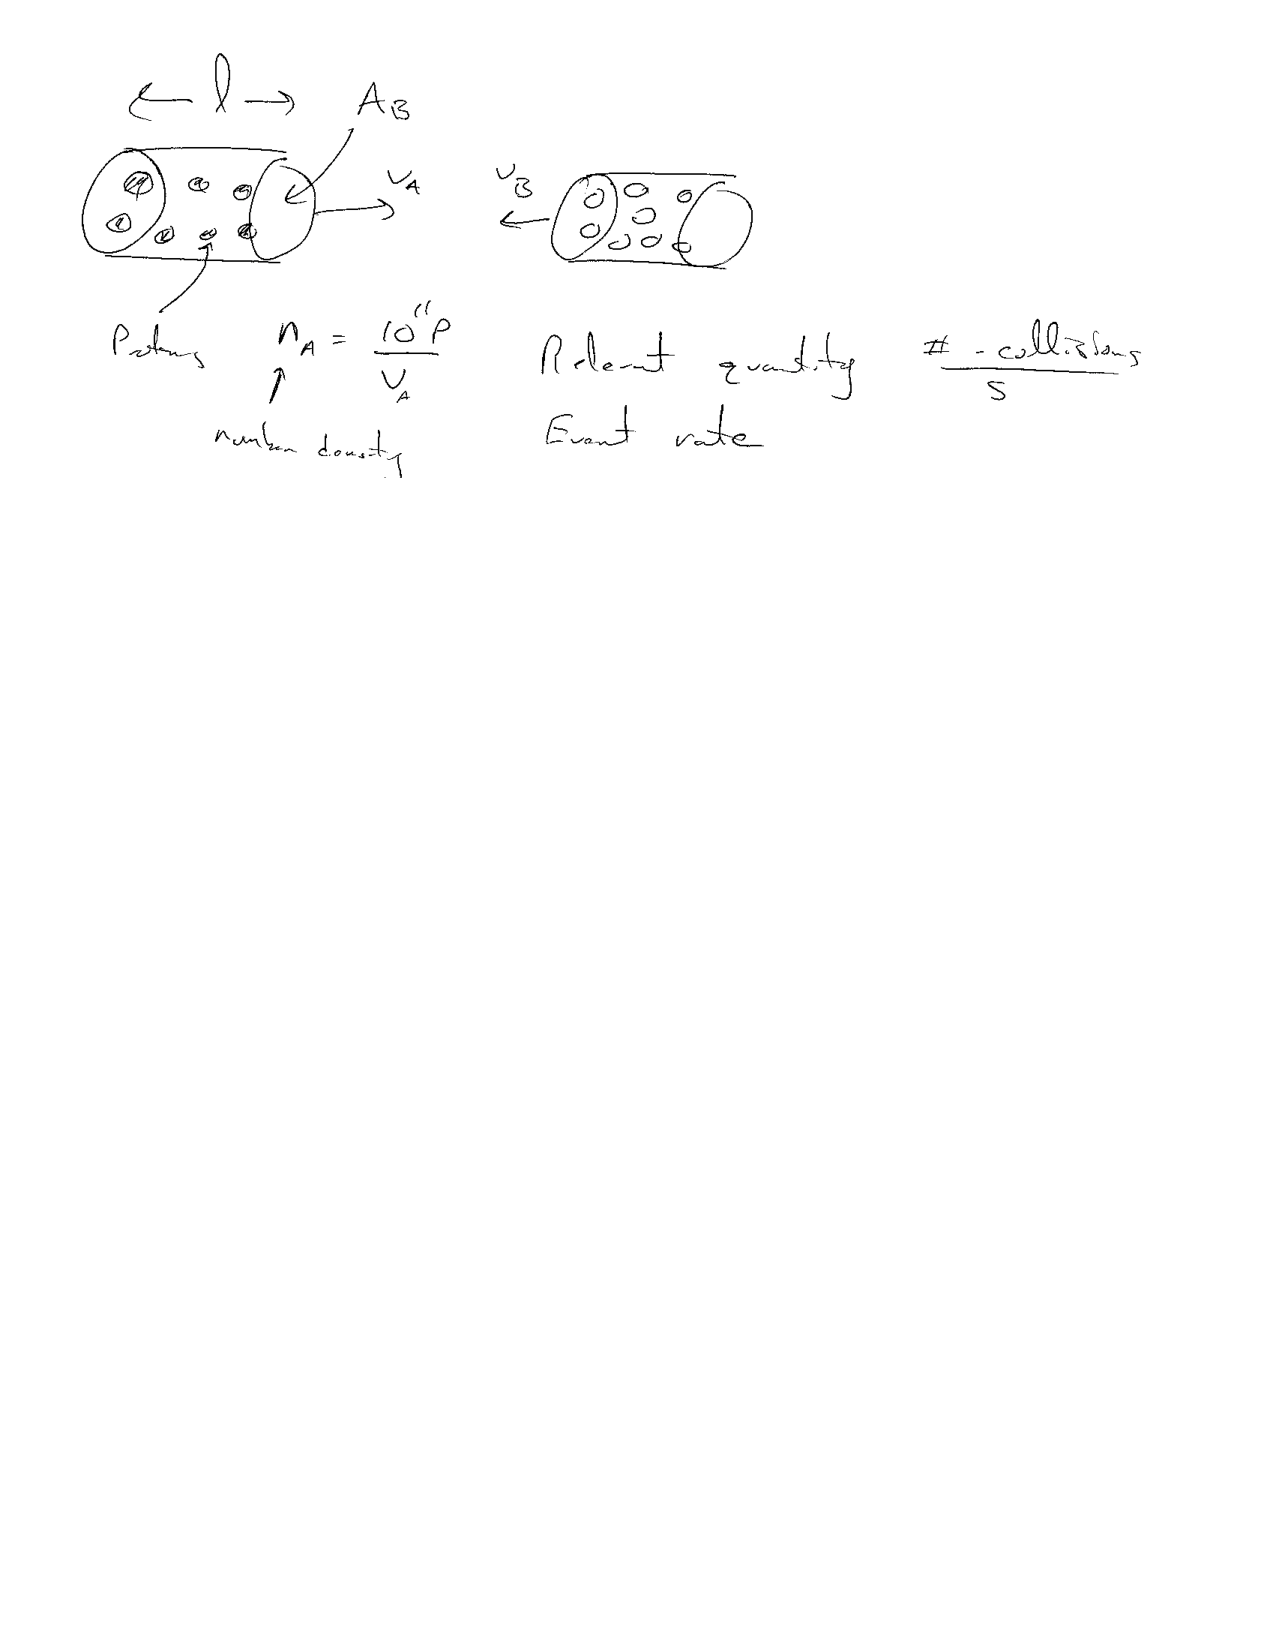
\includegraphics[width=1.0\textwidth]{./bunches.pdf}



Think about a slice of bunch ``B''.

The number of protons in bunch A that it sees per time is 

\be
\frac{N_A}{t} = n_A \cdot \underbrace{A_B \cdot |v_A - v_B|}_{\frac{\rmt{Volume}}{\rmt{time}} \rmt{of A that passes through B}}
\ee

Now the number of protons in B that could interact is 

\be
N_B^{\rmt{eff}} = n_B \cdot \underbrace{l \cdot \sigma}_{\rmt{Volume of the protons}}
\ee

$\Rightarrow$

\be
\frac{\rmt{Events}}{\rmt{Time}} = \frac{N_A N_B^{\rmt{eff}}}{t} = \underbrace{n_A n_B A l |v_A - v_B|}_{\rmt{flux factor we thought about before}} \sigma
\ee

\bi
\item[-] Flux factor depends on how the LHC was build
\item[-] $\sigma$ is an intrisic physical observable
\ei

Integrated Luminosity  $\rmt{L} = \int dt L$


Number of events is given by $\rmt{N}=\rmt{L}\times \sigma$

\fbox{\begin{minipage}{\textwidth}
\textbf{Q: What is the flux factor at the LHC ?}\\

Flux Factor also called $L$ ``instantaneous luminosity''  or just ``luminosity''

\be
L = n_A n_B A l |v_A - v_B| = \frac{N_A N_B |v_A - v_B|}{\underbrace{Vol}_{\rmt{Vol. of bunch $= A_B \times l$}}}
\ee

Now $\sigma$ is fixed, so to maximize number of events collected, need to maximize $L$

\bi
\item[-] $N_A = N_B = N = 10^{11}$ (fixed)
\item[-] $|v_A - v_B| = 2c$ can get much higher!
\item[-] Vol $\sim A_B \cdot l$ 
\ei

At the LHC, acceleration is done with radio-frequency EM feild that fixes $l$ (Protons ride in the troughs of this feild)
The wavelength of this feild sets $l \sim \frac{c}{2 \times 400\ \rmt{MHz}} \sim \frac{3}{4} m$ 

The one handle we have is $A_B$, focusing magnets (quadruples) act like a lens near the collision points to squeeze the beam.
So far focusing magnets have achieved squeezing down to the radii of 10 $\mu m$! 
Width of a human hair. 

\be
A_B \sim 10^{-10}\ m^2
\ee

$\Rightarrow$  

\be
L = 2c \frac{N^2}{lA} \sim 10^{-36} cm^{-2}s^{-1}
\ee



\end{minipage}}

}
\end{document}


